\documentclass[a4paper, 10pt]{article}
\usepackage{geometry}
\usepackage{indentfirst}
\usepackage{amsmath}
\usepackage{amssymb}
\usepackage{graphicx}
\usepackage{subfigure}
\usepackage{enumerate}
\usepackage{listings}
\usepackage{appendix}
\usepackage{xcolor}
\usepackage{multirow}
\usepackage{algorithm}
\usepackage{algorithmicx}
\usepackage{algpseudocode}
\usepackage{amsmath}
\usepackage{hyperref}
\renewcommand{\algorithmicrequire}{\textbf{Input:}}
\renewcommand{\algorithmicensure}{\textbf{Output:}}
\lstset{
  numbers=left,
  numberstyle= \tiny,
  keywordstyle= \color{ blue!70},
  commentstyle= \color{red!50!green!50!blue!50},
  frame=shadowbox,
  rulesepcolor= \color{ red!20!green!20!blue!20} ,
  escapeinside=``,
  xleftmargin=1em,xrightmargin=0em, aboveskip=1em,
  framexleftmargin=2em,
  showstringspaces=false,
  showtabs=false,
  breaklines=true
}
\lstdefinelanguage{JavaScript}{
  keywords={typeof, new, true, false, catch, function, return, null, catch, switch, var, if, in, while, do, else, case, break},
  keywordstyle=\color{blue}\bfseries,
  ndkeywords={class, export, boolean, throw, implements, import, this},
  ndkeywordstyle=\color{darkgray}\bfseries,
  identifierstyle=\color{black},
  sensitive=false,
  comment=[l]{//},
  morecomment=[s]{/*}{*/},
  commentstyle=\color{purple}\ttfamily,
  stringstyle=\color{red}\ttfamily,
  morestring=[b]',
  morestring=[b]"
}

\hypersetup{backref,  
  colorlinks=true,
  linkcolor=blue
} 

\title{\textbf{Final Project: Search Author Online}}
\author{
  Zhan Xinyu, 517030910358\\
  Wang Zhongye, \\
  Xie Yichen, \\
  Yue Ye
}
\begin{document}
\maketitle
\pagebreak
\tableofcontents
\pagebreak

\section{Introduction}
\subsection{Report Overview}
%what are covered in this report
%later any one
\subsection{Special Specification}
%later. increases as we write the report
\section{Project Overview}
\subsection{Website Overview}
%website demo and functionality list
%wang
\subsection{Project Structure}
%project structure
%zhan
\subsubsection{Website Structure}
\paragraph{Pages}\
Our website mainly consist of 4 types of pages: \textit{Home Page}, \textit{Result Page}, \textit{Information Pages} and \textit{Stats Pages}.
\subparagraph{\textit{Home Page}} The entrance of the website. Users can launch queries from here.
\subparagraph{\textit{Result Page}} Presents the result of the query, either from the \textit{Home Page} or from the search box in the navigation bar.
\subparagraph{\textit{Information Page}} Displays the basic information of one entity (publications, coauthors, affiliations, conferences, etc).
\subparagraph{\textit{Stats Page}} Contains the visualization graphs and charts, and recommendations on \textit{Paper Stats}.
\\

These pages are organized into the structure showed in the following chart:
\begin{figure}[H]
  \centering
  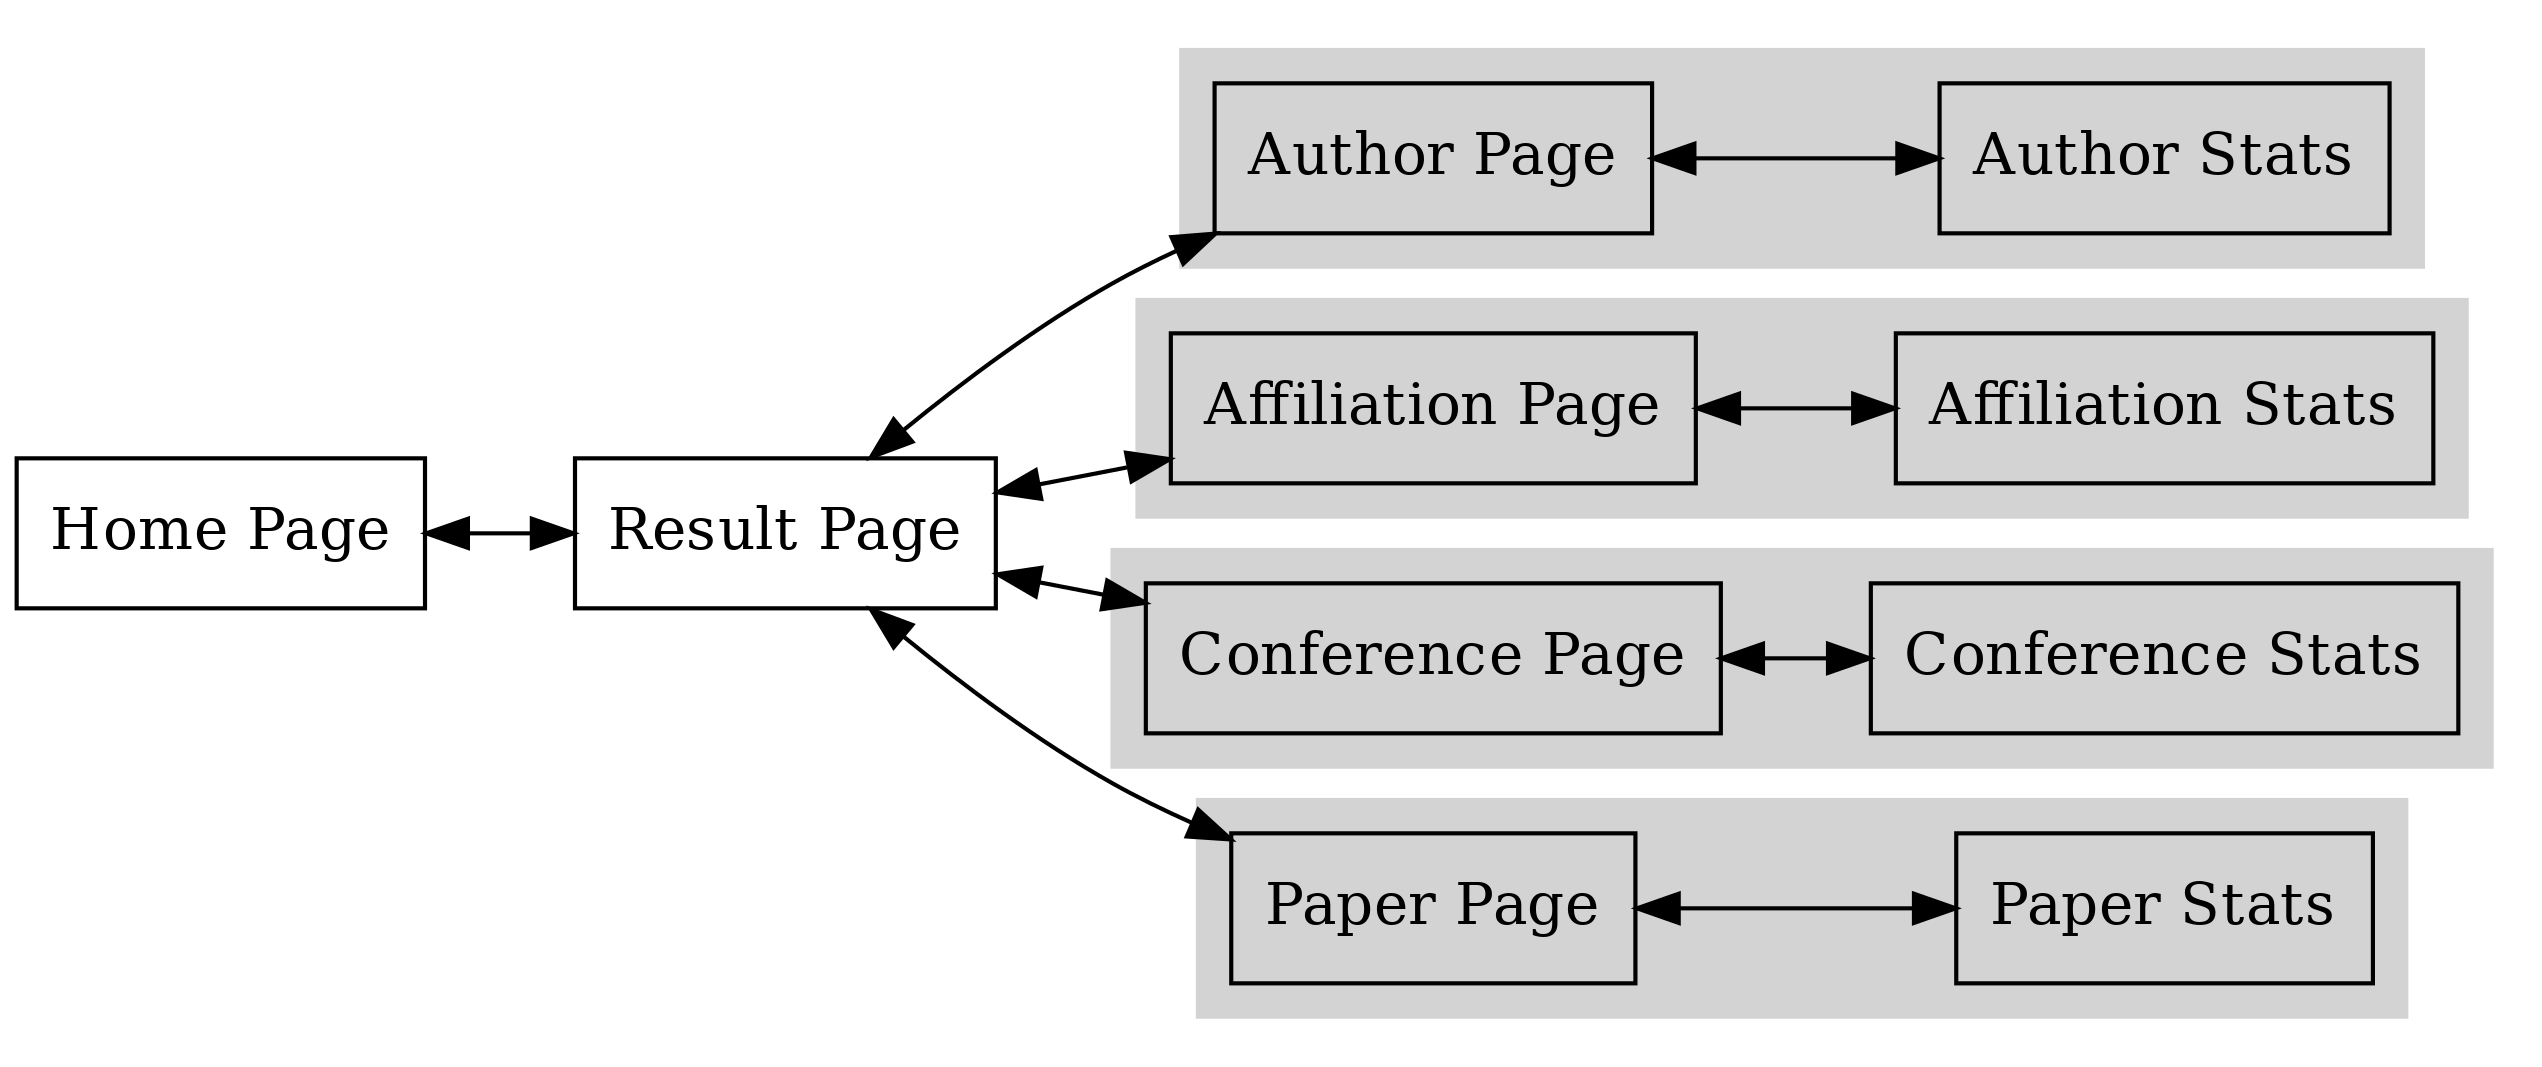
\includegraphics[width=\textwidth]{web_struct.png}
  \caption{The structure of the website}
  \label{fig:web_struct}
\end{figure}
As the chart shows, users will first visit our \textit{Home Page}, input some keywords, and press Enter. The page will redirect to \textit{Result Page}, and after user click one of the links present there, it will jump to the \textit{Information Pages}, which includes \textit{Author Page}, \textit{Affiliation Page}, \textit{Conference Page} and \textit{Paper Page}. From the navigation bar on the top of the \textit{Information Pages}, users can direct to the \textit{Stats Pages} corresponding to the \textit{Information Pages}. All pages can return to the \textit{Result Page} of the most recent query, and the \textit{Home Page}.

\subsubsection{Directory Structure}

In this project we use Code Igniter framework. The framework features MVC design pattern and a bunch of utility and helper funcitons. As a result, we mainly write codes and 
The directory structure of out project is like following:
\paragraph{application}\ 
This directory contains the php scripts that runs on the server and fulfill different jobs. These files mainly fall into three category: controllers, models and views, which follows the MVC design pattern.
\paragraph{assets}\


\subsubsection{Request Process Procedure}
The \textit{Result Page}, \textit{Information Pages} and \textit{Stats Pages} all involves many dynamic content loaded by js scripts from client side. To keep things simple, we design a standard and uniform request process procedure, and write some utilitiy functions for it.
The procedure is showed as follows:
\begin{figure}[H]
  \centering
  \caption{Request Process Procedure}
  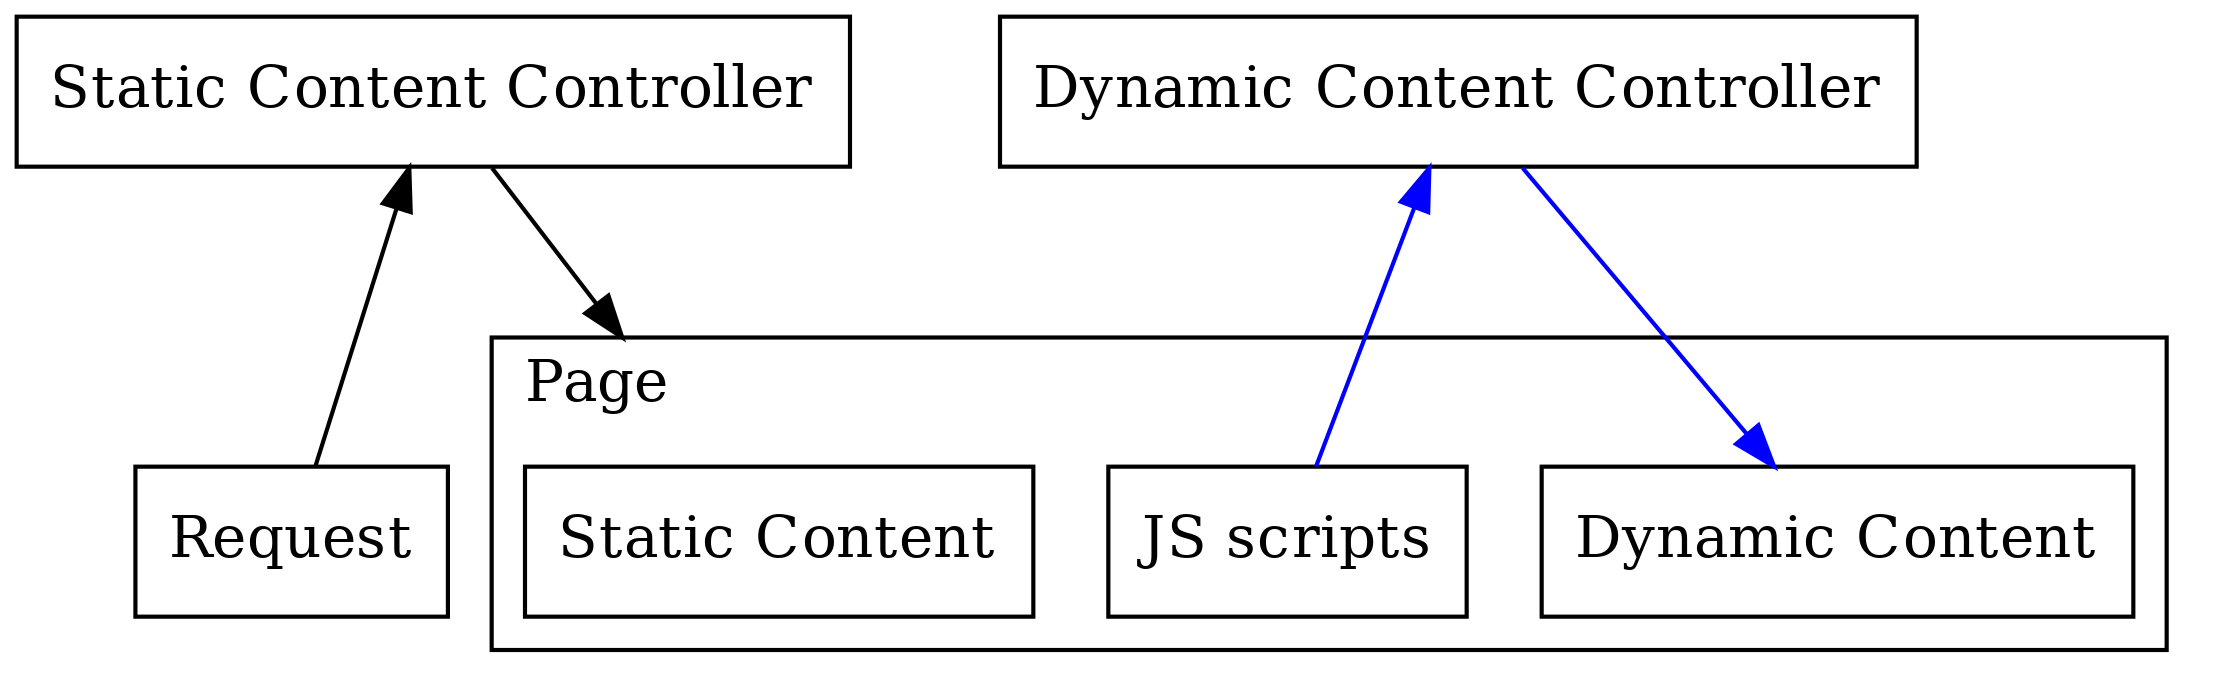
\includegraphics[width=\textwidth]{r_p_p.png}
  \label{fig:r_p_p}
\end{figure}

\subsubsection{Thirdparty packages and libraries}
\subsection{Project Organization}
%our github cooperation, workload division and building process can be demonstrated here
%zhan
\subsubsection{Workload Division}
\paragraph{Zhan Xinyu} Project structure; Website backend; Utility functions.
\paragraph{Wang Zhongye} Webpage Design; Website frontend, including css and js; Visualization charts.
\paragraph{Xie Yichen} Label Extraction; Page Recommendation. 
\paragraph{Yue Ye} Visualization backend; Slides.
\subsubsection{Collaboration with Git and Github}
To share code and synchronize 
\subsubsection{Website Deploy}
\section{Frontend Implementation}
%frontend implementation
%wang
%the interface of back-ends might be mentioned like "The implementation of this functionality will be illustrated in the following sections."
\subsection{Overview}
\subsection{UI Design}
\subsection{Data Visualization}
\section{Functionality Implementation}
%functionality(back-ends) implementation
%except wang
\subsection{Backend Implementation}
\subsection{Visualization Implementation}
\subsection{Label Extraction}
\subsection{Paper Recommendation}
\section{Future Work}
%future work
%later any one
\section{Conclusion}
%restated what we have accomplished
%later any one

\newpage
\begin{appendices}
  %depends
\end{appendices}
\end{document}
